% Created by tikzDevice version 0.7.0 on 2015-09-08 11:44:23
% !TEX encoding = UTF-8 Unicode
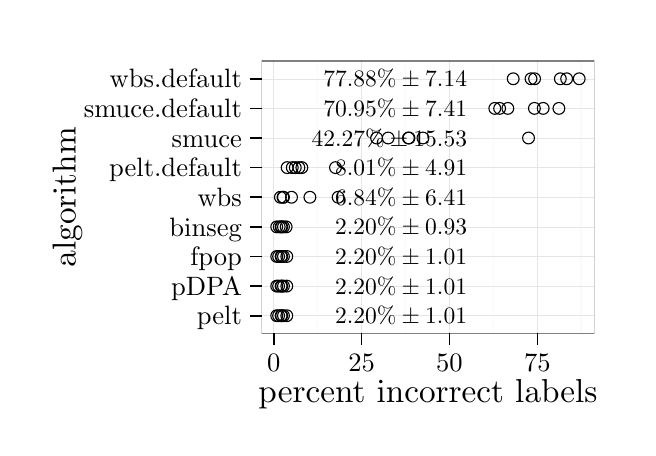
\begin{tikzpicture}[x=1pt,y=1pt]
\definecolor[named]{fillColor}{rgb}{1.00,1.00,1.00}
\path[use as bounding box,fill=fillColor,fill opacity=0.00] (0,0) rectangle (216.81,144.54);
\begin{scope}
\path[clip] (  0.00,  0.00) rectangle (216.81,144.54);
\definecolor[named]{drawColor}{rgb}{1.00,1.00,1.00}
\definecolor[named]{fillColor}{rgb}{1.00,1.00,1.00}

\path[draw=drawColor,line width= 0.6pt,line join=round,line cap=round,fill=fillColor] ( -0.00,  0.00) rectangle (216.81,144.54);
\end{scope}
\begin{scope}
\path[clip] ( 84.53, 34.03) rectangle (204.76,132.50);
\definecolor[named]{fillColor}{rgb}{1.00,1.00,1.00}

\path[fill=fillColor] ( 84.53, 34.03) rectangle (204.77,132.50);
\definecolor[named]{drawColor}{rgb}{0.98,0.98,0.98}

\path[draw=drawColor,line width= 0.6pt,line join=round] (104.77, 34.03) --
	(104.77,132.50);

\path[draw=drawColor,line width= 0.6pt,line join=round] (136.53, 34.03) --
	(136.53,132.50);

\path[draw=drawColor,line width= 0.6pt,line join=round] (168.29, 34.03) --
	(168.29,132.50);

\path[draw=drawColor,line width= 0.6pt,line join=round] (200.05, 34.03) --
	(200.05,132.50);
\definecolor[named]{drawColor}{rgb}{0.90,0.90,0.90}

\path[draw=drawColor,line width= 0.2pt,line join=round] ( 84.53, 40.46) --
	(204.76, 40.46);

\path[draw=drawColor,line width= 0.2pt,line join=round] ( 84.53, 51.16) --
	(204.76, 51.16);

\path[draw=drawColor,line width= 0.2pt,line join=round] ( 84.53, 61.86) --
	(204.76, 61.86);

\path[draw=drawColor,line width= 0.2pt,line join=round] ( 84.53, 72.56) --
	(204.76, 72.56);

\path[draw=drawColor,line width= 0.2pt,line join=round] ( 84.53, 83.26) --
	(204.76, 83.26);

\path[draw=drawColor,line width= 0.2pt,line join=round] ( 84.53, 93.97) --
	(204.76, 93.97);

\path[draw=drawColor,line width= 0.2pt,line join=round] ( 84.53,104.67) --
	(204.76,104.67);

\path[draw=drawColor,line width= 0.2pt,line join=round] ( 84.53,115.37) --
	(204.76,115.37);

\path[draw=drawColor,line width= 0.2pt,line join=round] ( 84.53,126.07) --
	(204.76,126.07);

\path[draw=drawColor,line width= 0.2pt,line join=round] ( 88.89, 34.03) --
	( 88.89,132.50);

\path[draw=drawColor,line width= 0.2pt,line join=round] (120.65, 34.03) --
	(120.65,132.50);

\path[draw=drawColor,line width= 0.2pt,line join=round] (152.41, 34.03) --
	(152.41,132.50);

\path[draw=drawColor,line width= 0.2pt,line join=round] (184.17, 34.03) --
	(184.17,132.50);
\definecolor[named]{drawColor}{rgb}{0.00,0.00,0.00}

\node[text=drawColor,anchor=base east,inner sep=0pt, outer sep=0pt, scale=  0.85] at (158.76, 37.53) {$2.20\% \pm 1.01$};

\node[text=drawColor,anchor=base east,inner sep=0pt, outer sep=0pt, scale=  0.85] at (158.76, 48.23) {$2.20\% \pm 1.01$};

\node[text=drawColor,anchor=base east,inner sep=0pt, outer sep=0pt, scale=  0.85] at (158.76, 58.93) {$2.20\% \pm 1.01$};

\node[text=drawColor,anchor=base east,inner sep=0pt, outer sep=0pt, scale=  0.85] at (158.76, 69.63) {$2.20\% \pm 0.93$};

\node[text=drawColor,anchor=base east,inner sep=0pt, outer sep=0pt, scale=  0.85] at (158.76, 80.34) {$6.84\% \pm 6.41$};

\node[text=drawColor,anchor=base east,inner sep=0pt, outer sep=0pt, scale=  0.85] at (158.76, 91.04) {$8.01\% \pm 4.91$};

\node[text=drawColor,anchor=base east,inner sep=0pt, outer sep=0pt, scale=  0.85] at (158.76,101.74) {$42.27\% \pm 15.53$};

\node[text=drawColor,anchor=base east,inner sep=0pt, outer sep=0pt, scale=  0.85] at (158.76,112.44) {$70.95\% \pm 7.41$};

\node[text=drawColor,anchor=base east,inner sep=0pt, outer sep=0pt, scale=  0.85] at (158.76,123.15) {$77.88\% \pm 7.14$};

\path[draw=drawColor,line width= 0.4pt,line join=round,line cap=round] ( 91.58, 40.46) circle (  2.13);

\path[draw=drawColor,line width= 0.4pt,line join=round,line cap=round] ( 92.43, 40.46) circle (  2.13);

\path[draw=drawColor,line width= 0.4pt,line join=round,line cap=round] ( 89.99, 40.46) circle (  2.13);

\path[draw=drawColor,line width= 0.4pt,line join=round,line cap=round] ( 91.79, 40.46) circle (  2.13);

\path[draw=drawColor,line width= 0.4pt,line join=round,line cap=round] ( 90.67, 40.46) circle (  2.13);

\path[draw=drawColor,line width= 0.4pt,line join=round,line cap=round] ( 93.63, 40.46) circle (  2.13);

\path[draw=drawColor,line width= 0.4pt,line join=round,line cap=round] ( 91.58, 51.16) circle (  2.13);

\path[draw=drawColor,line width= 0.4pt,line join=round,line cap=round] ( 92.43, 51.16) circle (  2.13);

\path[draw=drawColor,line width= 0.4pt,line join=round,line cap=round] ( 89.99, 51.16) circle (  2.13);

\path[draw=drawColor,line width= 0.4pt,line join=round,line cap=round] ( 91.79, 51.16) circle (  2.13);

\path[draw=drawColor,line width= 0.4pt,line join=round,line cap=round] ( 90.67, 51.16) circle (  2.13);

\path[draw=drawColor,line width= 0.4pt,line join=round,line cap=round] ( 93.63, 51.16) circle (  2.13);

\path[draw=drawColor,line width= 0.4pt,line join=round,line cap=round] ( 91.58, 61.86) circle (  2.13);

\path[draw=drawColor,line width= 0.4pt,line join=round,line cap=round] ( 92.43, 61.86) circle (  2.13);

\path[draw=drawColor,line width= 0.4pt,line join=round,line cap=round] ( 89.99, 61.86) circle (  2.13);

\path[draw=drawColor,line width= 0.4pt,line join=round,line cap=round] ( 91.79, 61.86) circle (  2.13);

\path[draw=drawColor,line width= 0.4pt,line join=round,line cap=round] ( 90.67, 61.86) circle (  2.13);

\path[draw=drawColor,line width= 0.4pt,line join=round,line cap=round] ( 93.63, 61.86) circle (  2.13);

\path[draw=drawColor,line width= 0.4pt,line join=round,line cap=round] ( 91.58, 72.56) circle (  2.13);

\path[draw=drawColor,line width= 0.4pt,line join=round,line cap=round] ( 92.43, 72.56) circle (  2.13);

\path[draw=drawColor,line width= 0.4pt,line join=round,line cap=round] ( 89.99, 72.56) circle (  2.13);

\path[draw=drawColor,line width= 0.4pt,line join=round,line cap=round] ( 91.79, 72.56) circle (  2.13);

\path[draw=drawColor,line width= 0.4pt,line join=round,line cap=round] ( 90.89, 72.56) circle (  2.13);

\path[draw=drawColor,line width= 0.4pt,line join=round,line cap=round] ( 93.40, 72.56) circle (  2.13);

\path[draw=drawColor,line width= 0.4pt,line join=round,line cap=round] (112.19, 83.26) circle (  2.13);

\path[draw=drawColor,line width= 0.4pt,line join=round,line cap=round] ( 92.43, 83.26) circle (  2.13);

\path[draw=drawColor,line width= 0.4pt,line join=round,line cap=round] ( 91.32, 83.26) circle (  2.13);

\path[draw=drawColor,line width= 0.4pt,line join=round,line cap=round] ( 92.24, 83.26) circle (  2.13);

\path[draw=drawColor,line width= 0.4pt,line join=round,line cap=round] ( 95.34, 83.26) circle (  2.13);

\path[draw=drawColor,line width= 0.4pt,line join=round,line cap=round] (101.98, 83.26) circle (  2.13);

\path[draw=drawColor,line width= 0.4pt,line join=round,line cap=round] ( 95.61, 93.97) circle (  2.13);

\path[draw=drawColor,line width= 0.4pt,line join=round,line cap=round] ( 99.07, 93.97) circle (  2.13);

\path[draw=drawColor,line width= 0.4pt,line join=round,line cap=round] ( 93.76, 93.97) circle (  2.13);

\path[draw=drawColor,line width= 0.4pt,line join=round,line cap=round] ( 96.70, 93.97) circle (  2.13);

\path[draw=drawColor,line width= 0.4pt,line join=round,line cap=round] ( 98.01, 93.97) circle (  2.13);

\path[draw=drawColor,line width= 0.4pt,line join=round,line cap=round] (111.23, 93.97) circle (  2.13);

\path[draw=drawColor,line width= 0.4pt,line join=round,line cap=round] (180.98,104.67) circle (  2.13);

\path[draw=drawColor,line width= 0.4pt,line join=round,line cap=round] (126.07,104.67) circle (  2.13);

\path[draw=drawColor,line width= 0.4pt,line join=round,line cap=round] (137.58,104.67) circle (  2.13);

\path[draw=drawColor,line width= 0.4pt,line join=round,line cap=round] (137.79,104.67) circle (  2.13);

\path[draw=drawColor,line width= 0.4pt,line join=round,line cap=round] (130.27,104.67) circle (  2.13);

\path[draw=drawColor,line width= 0.4pt,line join=round,line cap=round] (142.82,104.67) circle (  2.13);

\path[draw=drawColor,line width= 0.4pt,line join=round,line cap=round] (191.96,115.37) circle (  2.13);

\path[draw=drawColor,line width= 0.4pt,line join=round,line cap=round] (168.79,115.37) circle (  2.13);

\path[draw=drawColor,line width= 0.4pt,line join=round,line cap=round] (186.28,115.37) circle (  2.13);

\path[draw=drawColor,line width= 0.4pt,line join=round,line cap=round] (183.11,115.37) circle (  2.13);

\path[draw=drawColor,line width= 0.4pt,line join=round,line cap=round] (170.54,115.37) circle (  2.13);

\path[draw=drawColor,line width= 0.4pt,line join=round,line cap=round] (173.51,115.37) circle (  2.13);

\path[draw=drawColor,line width= 0.4pt,line join=round,line cap=round] (192.47,126.07) circle (  2.13);

\path[draw=drawColor,line width= 0.4pt,line join=round,line cap=round] (181.88,126.07) circle (  2.13);

\path[draw=drawColor,line width= 0.4pt,line join=round,line cap=round] (199.30,126.07) circle (  2.13);

\path[draw=drawColor,line width= 0.4pt,line join=round,line cap=round] (194.76,126.07) circle (  2.13);

\path[draw=drawColor,line width= 0.4pt,line join=round,line cap=round] (183.17,126.07) circle (  2.13);

\path[draw=drawColor,line width= 0.4pt,line join=round,line cap=round] (175.44,126.07) circle (  2.13);
\definecolor[named]{drawColor}{rgb}{0.50,0.50,0.50}

\path[draw=drawColor,line width= 0.6pt,line join=round,line cap=round] ( 84.53, 34.03) rectangle (204.77,132.50);
\end{scope}
\begin{scope}
\path[clip] (  0.00,  0.00) rectangle (216.81,144.54);
\definecolor[named]{drawColor}{rgb}{0.00,0.00,0.00}

\node[text=drawColor,anchor=base east,inner sep=0pt, outer sep=0pt, scale=  0.96] at ( 77.42, 37.15) {pelt};

\node[text=drawColor,anchor=base east,inner sep=0pt, outer sep=0pt, scale=  0.96] at ( 77.42, 47.85) {pDPA};

\node[text=drawColor,anchor=base east,inner sep=0pt, outer sep=0pt, scale=  0.96] at ( 77.42, 58.55) {fpop};

\node[text=drawColor,anchor=base east,inner sep=0pt, outer sep=0pt, scale=  0.96] at ( 77.42, 69.26) {binseg};

\node[text=drawColor,anchor=base east,inner sep=0pt, outer sep=0pt, scale=  0.96] at ( 77.42, 79.96) {wbs};

\node[text=drawColor,anchor=base east,inner sep=0pt, outer sep=0pt, scale=  0.96] at ( 77.42, 90.66) {pelt.default};

\node[text=drawColor,anchor=base east,inner sep=0pt, outer sep=0pt, scale=  0.96] at ( 77.42,101.36) {smuce};

\node[text=drawColor,anchor=base east,inner sep=0pt, outer sep=0pt, scale=  0.96] at ( 77.42,112.07) {smuce.default};

\node[text=drawColor,anchor=base east,inner sep=0pt, outer sep=0pt, scale=  0.96] at ( 77.42,122.77) {wbs.default};
\end{scope}
\begin{scope}
\path[clip] (  0.00,  0.00) rectangle (216.81,144.54);
\definecolor[named]{drawColor}{rgb}{0.00,0.00,0.00}

\path[draw=drawColor,line width= 0.6pt,line join=round] ( 80.26, 40.46) --
	( 84.53, 40.46);

\path[draw=drawColor,line width= 0.6pt,line join=round] ( 80.26, 51.16) --
	( 84.53, 51.16);

\path[draw=drawColor,line width= 0.6pt,line join=round] ( 80.26, 61.86) --
	( 84.53, 61.86);

\path[draw=drawColor,line width= 0.6pt,line join=round] ( 80.26, 72.56) --
	( 84.53, 72.56);

\path[draw=drawColor,line width= 0.6pt,line join=round] ( 80.26, 83.26) --
	( 84.53, 83.26);

\path[draw=drawColor,line width= 0.6pt,line join=round] ( 80.26, 93.97) --
	( 84.53, 93.97);

\path[draw=drawColor,line width= 0.6pt,line join=round] ( 80.26,104.67) --
	( 84.53,104.67);

\path[draw=drawColor,line width= 0.6pt,line join=round] ( 80.26,115.37) --
	( 84.53,115.37);

\path[draw=drawColor,line width= 0.6pt,line join=round] ( 80.26,126.07) --
	( 84.53,126.07);
\end{scope}
\begin{scope}
\path[clip] (  0.00,  0.00) rectangle (216.81,144.54);
\definecolor[named]{drawColor}{rgb}{0.00,0.00,0.00}

\path[draw=drawColor,line width= 0.6pt,line join=round] ( 88.89, 29.77) --
	( 88.89, 34.03);

\path[draw=drawColor,line width= 0.6pt,line join=round] (120.65, 29.77) --
	(120.65, 34.03);

\path[draw=drawColor,line width= 0.6pt,line join=round] (152.41, 29.77) --
	(152.41, 34.03);

\path[draw=drawColor,line width= 0.6pt,line join=round] (184.17, 29.77) --
	(184.17, 34.03);
\end{scope}
\begin{scope}
\path[clip] (  0.00,  0.00) rectangle (216.81,144.54);
\definecolor[named]{drawColor}{rgb}{0.00,0.00,0.00}

\node[text=drawColor,anchor=base,inner sep=0pt, outer sep=0pt, scale=  0.96] at ( 88.89, 20.31) {0};

\node[text=drawColor,anchor=base,inner sep=0pt, outer sep=0pt, scale=  0.96] at (120.65, 20.31) {25};

\node[text=drawColor,anchor=base,inner sep=0pt, outer sep=0pt, scale=  0.96] at (152.41, 20.31) {50};

\node[text=drawColor,anchor=base,inner sep=0pt, outer sep=0pt, scale=  0.96] at (184.17, 20.31) {75};
\end{scope}
\begin{scope}
\path[clip] (  0.00,  0.00) rectangle (216.81,144.54);
\definecolor[named]{drawColor}{rgb}{0.00,0.00,0.00}

\node[text=drawColor,anchor=base,inner sep=0pt, outer sep=0pt, scale=  1.20] at (144.65,  9.03) {percent incorrect labels};
\end{scope}
\begin{scope}
\path[clip] (  0.00,  0.00) rectangle (216.81,144.54);
\definecolor[named]{drawColor}{rgb}{0.00,0.00,0.00}

\node[text=drawColor,rotate= 90.00,anchor=base,inner sep=0pt, outer sep=0pt, scale=  1.20] at ( 17.30, 83.26) {algorithm};
\end{scope}
\end{tikzpicture}
